\subsection{A scale-free He3 placement-response curve}
\label{sec:he3-chart-12}

The complete 192 source's retained four-pole intrinsic factor gives a
response chart independent of an absolute energy scale. Reuse
$r=\tau/\delta$, $a_k=(1+4kr)^{-1}$ and $S_j=\sum_{k=0}^3a_k^j$ from
\eqref{eq:he3-secular-new}. For the normalized vector $a/\sqrt{S_2}$,
the rank-one incidence projector $P=\mathbf1\mathbf1^T/4$ has
\begin{equation}
\begin{gathered}
 \theta=\tau/\epsilon=rS_1/4,\quad d=\delta/\epsilon=S_1/4,\\
 p=S_1^2/(4S_2),\qquad q=4\sum_{k=0}^3ka_k^2/S_2.
\end{gathered}
\end{equation}
Here $q$ is the placement-response observable, distinct from the atomic
receiver square also denoted $q$ in Chapter~XIV. The factor equation
$(4\theta\diag(k)-P)a=-da$ implies the exact cost identity
\begin{equation}
 \theta q=p-d,
\label{eq:he3-chart-12}
\end{equation}
because $S_1-S_2=4r\sum ka_k^2$. It is the original formation cost divided
by $\epsilon$, not an extra energy gain.\samref{REF12_FOUR}

Since $(ra_k)'=a_k^2$, $\theta'=S_2/4>0$. Strict Cauchy gives
$p'/p=(2/r)(S_2/S_1-S_3/S_2)<0$ for $r>0$.
Differentiating the normalized $a_k^2$ weights makes $q'/4$ the covariance
of $k$ with $-8k/(1+4kr)$, also strictly negative. Thus $\theta$
parametrizes the curve uniquely: $p$ decreases from one to $1/4$ and $q$
from six to zero. The endpoint expansions are
$1-p=20\theta^2+O(\theta^3)$ and
$p-1/4=11/(192\theta)+O(\theta^{-2})$.

Six rational $r$ values $0,1/100,1/10,1,10,100$ have separately retained
zero factor/cost residuals. These checks anchor the chart; they do not
replace the inherited full192 spectral proof. Inverse calibration is
well conditioned only on compact interior ranges. A measurement must
identify the projector/detuning and prepare this intrinsic factor, or pay
joint-field backreaction. Neither a joint-ground susceptibility nor a
physical $\tau$ is inferred from this intrinsic curve alone.

\begin{figure}[htbp]\centering
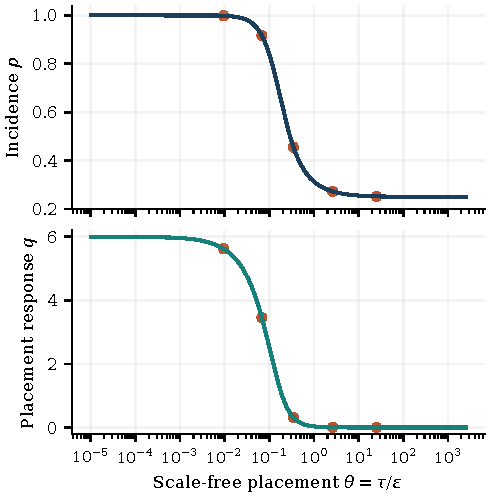
\includegraphics[width=\columnwidth]{refinement_20261112/figures/he3_chart.pdf}
\caption{The exact intrinsic He3 response chart. Curves use the same
four-pole factor as the complete 192 theorem; dots are the positive
rational-$r$ checkpoints. The atomic receiver variable is unrelated to
the placement observable $q$ plotted here.}
\label{fig:he3-chart-12}
\end{figure}
